This chapter will discuss the evaluation process of the application including testing, evaluation experiments, and, the results gathered.

\section{Testing}


\section{Experiment}
To evaluate the application an experiment was planned to gather user feedback, and, measure usability. The initial plan was to have participants download the application, then complete the experiment. However, it was discovered that if the user was using an iOS device, they could not simply access a link and download the application. Apple's TestFlight platform is designed to alleviate this struggle by allowing developers to upload builds and have users download the application from there, this however is part of Apple's developer program, a paid service, so was not suitable. It was decided at this stage that two similar experiments were to be run, one in person on a device with the application installed, and, an online survey showcasing application screenshots and recordings. This approach was taken to ensure there was a sufficient number of participants in the evaluation, due to the in person experiment being run solely on one device. 

\subsection*{Ethics}
Both experiments were performed in line with the University of Glasgow's School of Computer Science ethics checklist \cite{ethics}. All participants consented, were allowed to ask any questions, and, were provided with contact details. A brief,  and, debrief were provided to all participants stating the aims of the experiment and reminding the participant they are free to stop at any time.

\subsection*{Participants}
A wide variety of ages, genders, and technological backgrounds were consulted in this evaluation. The majority of the participants were part of the target demographic for the application, aged eighteen to thirty. 

\subsection{In Person}
The goals of the in person evaluation were to measure the usability of application and gather user feedback on their experience. The participant was first presented with some introductory questions to gain some initial opinions on the problem this application aims to solve, usage of similar concepts, and, the concept of this application (see \ref{appendix:introQns}).
Evaluating usability comprised of the participant completing a set of tasks, after each task the participant was asked the single ease question \cite{seq}, \textit{How difficult did you find this task?}. This was answered through a five point Likert scale ranging from very difficult, to very easy. 
The tasks were designed to incorporate all key areas of the application, creating accounts and groups, adding friends, and, customizing the user experience (see \ref{appendix:tasks}).

This was further complemented by the use of the system usability scale (SUS) \cite{sus}, the industry standard for evaluating the usability of products. The SUS comprises of ten questions answered through a five point Likert scale ranging from strongly disagree, to strongly agree (see \ref{appendix:susQns}). This was completed by the participant after all the tasks had been completed.

After completion the participant was asked some concluding questions used to gather user feedback after usage of the application (see \ref{appendix:concludQns}). 
For an example survey response see \cite{evalRespWApp}.

\subsection{Online}
The online evaluation consisted of the same introductory, and, concluding questions but with a change to the usability evaluation. As the user would not have direct interaction with the application, the usability study performed during the in person evaluation was not suitable. Instead, two screen recordings of an example user interacting with the application were created, alongside Likert scale questions regarding the video content (see \ref{appendix:vidQns}). The participant was then asked to answer some general questions regarding the application and were given several screenshots of the application for reference (see \ref{appendix:onlineGenQns}). Although it was not possible to use the system usability scale, questions were designed to be very similar to gather useful results. For an example survey response see \cite{evalRespNoApp}. 

\section{Results}
In total there were 32 participants in the experiment, 24 online, and, 8 in person. The combination of both an in person, and, online evaluation allowed the gathering of a suitable number of responses which would not have been possible with a purely in person evaluation.

\subsection{Introductory \& Conluding Questions}
The responses to the introductory, and, concluding questions have been combined and presented below. The results from the introductory questions \ref{fig:introAns}, confirm that people do have issues with planning activities due to being unaware of their status, the problem this application aims to solve. Participants show a clear interest in the application concept with 91\% being likely to use an app to graphically see their friends status. 

\begin{figure}[H]

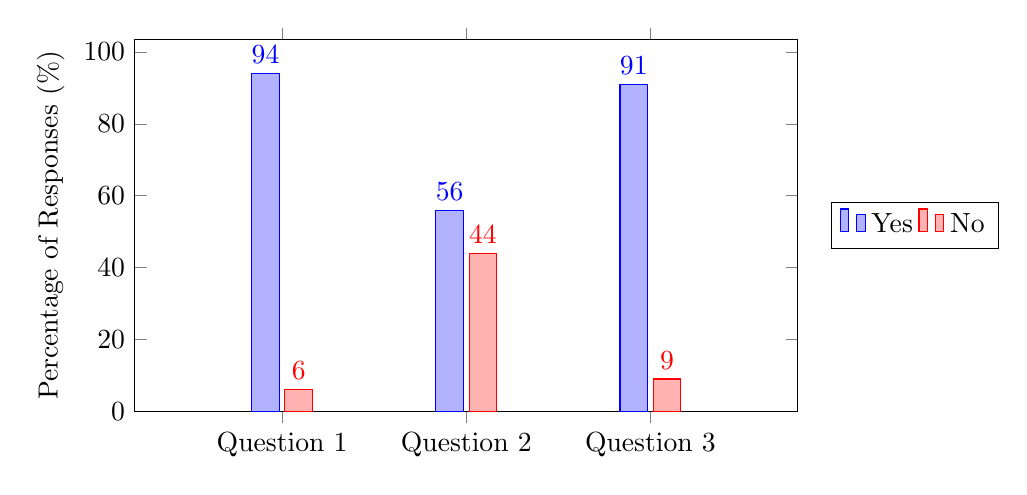
\begin{tikzpicture}  
\begin{axis}  
[  
    ybar,
    width=10cm,
    height=6.3cm,
    enlarge x limits=0.4,     
    ylabel={Percentage of Responses (\%)},
    ymin=0,
    symbolic x coords={Question 1, Question 2, Question 3},  
    xtick=data,  
    nodes near coords,  
    nodes near coords align={vertical},  
    legend style={at={(1.05,0.5)},anchor=west, legend columns=-1},
    ]  
\addplot coordinates {(Question 1, 94) (Question 2, 56) (Question 3, 91)};
\addplot coordinates {(Question 1, 6) (Question 2, 44) (Question 3, 9)};  
\legend{Yes, No}  
  
\end{axis}  
\end{tikzpicture} 
\begin{enumerate}
    \item Do you have issues with planning activities due to being unaware of your friends status?
    \item Do you use snapchat maps or life360 for example to see what your friends are up to?
    \item Would you be likely to use an app to graphically see your friends status?
\end{enumerate}

\caption{Combined results of introductory questions}
\label{fig:introAns}
\end{figure}
\FloatBarrier

The results concluding both experiments show a clear trend of participant interest in the concept, and application itself with 84\% interested in the concept, and 66\% potentially would use the application. All  participants responded either yes, or, maybe with zero participants responding no to either of the questions.


\begin{figure}[H]

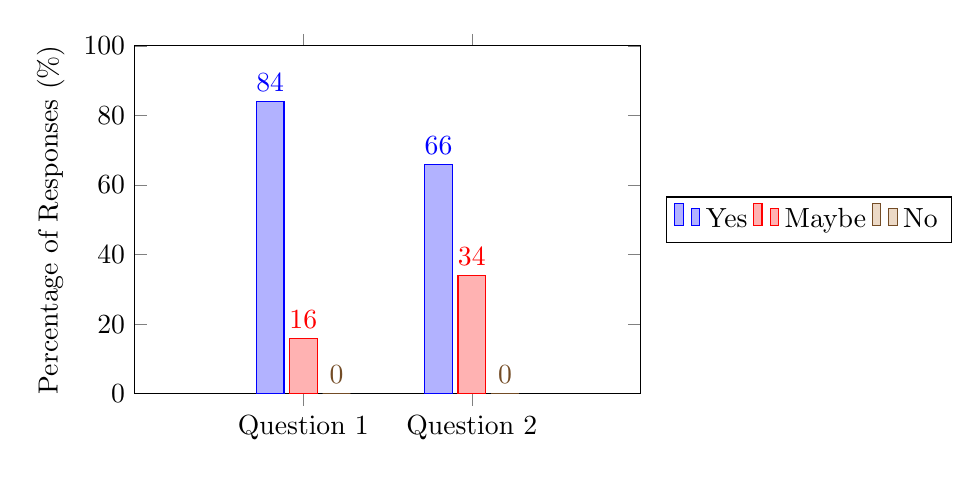
\begin{tikzpicture}  
\begin{axis}  
[  
    ybar,
    width=8cm,
    height=6cm,
    enlarge x limits=1,       
    ylabel={Percentage of Responses (\%)},
    ymin=0,
    ymax=100,
    symbolic x coords={Question 1, Question 2},  
    xtick=data,  
    nodes near coords,  
    nodes near coords align={vertical},  
    legend style={at={(1.05,0.5)},anchor=west, legend columns=-1},
    ]  
\addplot coordinates {(Question 1, 84) (Question 2, 66)};
\addplot coordinates {(Question 1, 16) (Question 2, 34)}; 
\addplot coordinates {(Question 1, 0) (Question 2, 0)}; 
\legend{Yes, Maybe, No}  
  
\end{axis}  
\end{tikzpicture} 
\begin{enumerate}
    \item After using the app are you interested in the concept?
    \item Would you potentially use such an app?
\end{enumerate}
\caption{Combined results of concluding questions}
\label{fig:conclAns}
\end{figure}
\FloatBarrier

\subsection{System Usability Scale}
The system usability scale was completed by 8 participants during the in person evaluation after the user had completed all of the tasks. Calculating the SUS score involves subtracting 1 from the responses to the positive questions, then, responses to the negative questions are subtracted from 5. These values are the summed together, and multiplied by 2.5 to give a SUS score in the range 0-100. The participant responses to each question, and, SUS score are shown in \ref{appendix:susQns}. The average SUS score taken from the responses from all participants is 84.38, obtaining the highest grade of A+ according to the grading scale proposed by James Lewis and Jeff Sauro \cite{susGrades}. These results are a reliable measure of system usability, portraying how participants were impressed by the usability of the application.

\subsection{Online Evaluation Questions}

\subsection{Participant Feedback}

\subsection{In Person Experiment Observations}

\section{Summary}